% Options for packages loaded elsewhere
\PassOptionsToPackage{unicode}{hyperref}
\PassOptionsToPackage{hyphens}{url}
%
\documentclass[
]{article}
\usepackage{amsmath,amssymb}
\usepackage{iftex}
\ifPDFTeX
  \usepackage[T1]{fontenc}
  \usepackage[utf8]{inputenc}
  \usepackage{textcomp} % provide euro and other symbols
\else % if luatex or xetex
  \usepackage{unicode-math} % this also loads fontspec
  \defaultfontfeatures{Scale=MatchLowercase}
  \defaultfontfeatures[\rmfamily]{Ligatures=TeX,Scale=1}
\fi
\usepackage{lmodern}
\ifPDFTeX\else
  % xetex/luatex font selection
\fi
% Use upquote if available, for straight quotes in verbatim environments
\IfFileExists{upquote.sty}{\usepackage{upquote}}{}
\IfFileExists{microtype.sty}{% use microtype if available
  \usepackage[]{microtype}
  \UseMicrotypeSet[protrusion]{basicmath} % disable protrusion for tt fonts
}{}
\makeatletter
\@ifundefined{KOMAClassName}{% if non-KOMA class
  \IfFileExists{parskip.sty}{%
    \usepackage{parskip}
  }{% else
    \setlength{\parindent}{0pt}
    \setlength{\parskip}{6pt plus 2pt minus 1pt}}
}{% if KOMA class
  \KOMAoptions{parskip=half}}
\makeatother
\usepackage{xcolor}
\usepackage[margin=1in]{geometry}
\usepackage{color}
\usepackage{fancyvrb}
\newcommand{\VerbBar}{|}
\newcommand{\VERB}{\Verb[commandchars=\\\{\}]}
\DefineVerbatimEnvironment{Highlighting}{Verbatim}{commandchars=\\\{\}}
% Add ',fontsize=\small' for more characters per line
\usepackage{framed}
\definecolor{shadecolor}{RGB}{248,248,248}
\newenvironment{Shaded}{\begin{snugshade}}{\end{snugshade}}
\newcommand{\AlertTok}[1]{\textcolor[rgb]{0.94,0.16,0.16}{#1}}
\newcommand{\AnnotationTok}[1]{\textcolor[rgb]{0.56,0.35,0.01}{\textbf{\textit{#1}}}}
\newcommand{\AttributeTok}[1]{\textcolor[rgb]{0.13,0.29,0.53}{#1}}
\newcommand{\BaseNTok}[1]{\textcolor[rgb]{0.00,0.00,0.81}{#1}}
\newcommand{\BuiltInTok}[1]{#1}
\newcommand{\CharTok}[1]{\textcolor[rgb]{0.31,0.60,0.02}{#1}}
\newcommand{\CommentTok}[1]{\textcolor[rgb]{0.56,0.35,0.01}{\textit{#1}}}
\newcommand{\CommentVarTok}[1]{\textcolor[rgb]{0.56,0.35,0.01}{\textbf{\textit{#1}}}}
\newcommand{\ConstantTok}[1]{\textcolor[rgb]{0.56,0.35,0.01}{#1}}
\newcommand{\ControlFlowTok}[1]{\textcolor[rgb]{0.13,0.29,0.53}{\textbf{#1}}}
\newcommand{\DataTypeTok}[1]{\textcolor[rgb]{0.13,0.29,0.53}{#1}}
\newcommand{\DecValTok}[1]{\textcolor[rgb]{0.00,0.00,0.81}{#1}}
\newcommand{\DocumentationTok}[1]{\textcolor[rgb]{0.56,0.35,0.01}{\textbf{\textit{#1}}}}
\newcommand{\ErrorTok}[1]{\textcolor[rgb]{0.64,0.00,0.00}{\textbf{#1}}}
\newcommand{\ExtensionTok}[1]{#1}
\newcommand{\FloatTok}[1]{\textcolor[rgb]{0.00,0.00,0.81}{#1}}
\newcommand{\FunctionTok}[1]{\textcolor[rgb]{0.13,0.29,0.53}{\textbf{#1}}}
\newcommand{\ImportTok}[1]{#1}
\newcommand{\InformationTok}[1]{\textcolor[rgb]{0.56,0.35,0.01}{\textbf{\textit{#1}}}}
\newcommand{\KeywordTok}[1]{\textcolor[rgb]{0.13,0.29,0.53}{\textbf{#1}}}
\newcommand{\NormalTok}[1]{#1}
\newcommand{\OperatorTok}[1]{\textcolor[rgb]{0.81,0.36,0.00}{\textbf{#1}}}
\newcommand{\OtherTok}[1]{\textcolor[rgb]{0.56,0.35,0.01}{#1}}
\newcommand{\PreprocessorTok}[1]{\textcolor[rgb]{0.56,0.35,0.01}{\textit{#1}}}
\newcommand{\RegionMarkerTok}[1]{#1}
\newcommand{\SpecialCharTok}[1]{\textcolor[rgb]{0.81,0.36,0.00}{\textbf{#1}}}
\newcommand{\SpecialStringTok}[1]{\textcolor[rgb]{0.31,0.60,0.02}{#1}}
\newcommand{\StringTok}[1]{\textcolor[rgb]{0.31,0.60,0.02}{#1}}
\newcommand{\VariableTok}[1]{\textcolor[rgb]{0.00,0.00,0.00}{#1}}
\newcommand{\VerbatimStringTok}[1]{\textcolor[rgb]{0.31,0.60,0.02}{#1}}
\newcommand{\WarningTok}[1]{\textcolor[rgb]{0.56,0.35,0.01}{\textbf{\textit{#1}}}}
\usepackage{graphicx}
\makeatletter
\def\maxwidth{\ifdim\Gin@nat@width>\linewidth\linewidth\else\Gin@nat@width\fi}
\def\maxheight{\ifdim\Gin@nat@height>\textheight\textheight\else\Gin@nat@height\fi}
\makeatother
% Scale images if necessary, so that they will not overflow the page
% margins by default, and it is still possible to overwrite the defaults
% using explicit options in \includegraphics[width, height, ...]{}
\setkeys{Gin}{width=\maxwidth,height=\maxheight,keepaspectratio}
% Set default figure placement to htbp
\makeatletter
\def\fps@figure{htbp}
\makeatother
\setlength{\emergencystretch}{3em} % prevent overfull lines
\providecommand{\tightlist}{%
  \setlength{\itemsep}{0pt}\setlength{\parskip}{0pt}}
\setcounter{secnumdepth}{-\maxdimen} % remove section numbering
\ifLuaTeX
  \usepackage{selnolig}  % disable illegal ligatures
\fi
\IfFileExists{bookmark.sty}{\usepackage{bookmark}}{\usepackage{hyperref}}
\IfFileExists{xurl.sty}{\usepackage{xurl}}{} % add URL line breaks if available
\urlstyle{same}
\hypersetup{
  pdftitle={aflevering},
  hidelinks,
  pdfcreator={LaTeX via pandoc}}

\title{aflevering}
\author{}
\date{\vspace{-2.5em}2023-10-17}

\begin{document}
\maketitle

\hypertarget{part-i}{%
\subsection{Part I}\label{part-i}}

\hypertarget{section}{%
\subsubsection{1.}\label{section}}

\begin{Shaded}
\begin{Highlighting}[]
\NormalTok{control }\OtherTok{\textless{}{-}}\NormalTok{ toxData }\SpecialCharTok{\%\textgreater{}\%} \FunctionTok{filter}\NormalTok{(conc }\SpecialCharTok{==} \DecValTok{0}\NormalTok{)}
\NormalTok{mod }\OtherTok{\textless{}{-}} \FunctionTok{lmer}\NormalTok{(fluorescence }\SpecialCharTok{\textasciitilde{}}\NormalTok{ day}\DecValTok{{-}1} \SpecialCharTok{+}\NormalTok{ (}\DecValTok{1}\SpecialCharTok{|}\NormalTok{plate) , }\AttributeTok{data =}\NormalTok{ control) }
\FunctionTok{confint}\NormalTok{(mod)}
\end{Highlighting}
\end{Shaded}

\begin{verbatim}
## Computing profile confidence intervals ...
\end{verbatim}

\begin{verbatim}
##            2.5 %    97.5 %
## .sig01  143.0122  441.2169
## .sigma  110.7260  166.1850
## day1    515.5940 1270.2631
## day2   2084.4615 2699.6218
## day3   2183.7303 2937.1447
\end{verbatim}

\hypertarget{section-1}{%
\subsubsection{2.}\label{section-1}}

Somewhat difference

\hypertarget{part-ii}{%
\subsection{Part II}\label{part-ii}}

\begin{Shaded}
\begin{Highlighting}[]
\NormalTok{mod }\OtherTok{\textless{}{-}} \FunctionTok{lmer}\NormalTok{(fluorescence }\SpecialCharTok{\textasciitilde{}}\NormalTok{ day}\SpecialCharTok{*}\NormalTok{concFac}\DecValTok{{-}1} \SpecialCharTok{+}\NormalTok{ (}\DecValTok{1}\SpecialCharTok{|}\NormalTok{plate) , }\AttributeTok{data =}\NormalTok{ toxData)}
\NormalTok{mod\_sqrt }\OtherTok{\textless{}{-}} \FunctionTok{lmer}\NormalTok{(}\FunctionTok{sqrt}\NormalTok{(fluorescence) }\SpecialCharTok{\textasciitilde{}}\NormalTok{ day}\SpecialCharTok{*}\NormalTok{concFac }\SpecialCharTok{+}\NormalTok{ (}\DecValTok{1}\SpecialCharTok{|}\NormalTok{plate) , }\AttributeTok{data =}\NormalTok{ toxData)}
\NormalTok{mod\_log }\OtherTok{\textless{}{-}} \FunctionTok{lmer}\NormalTok{(}\FunctionTok{log}\NormalTok{(fluorescence) }\SpecialCharTok{\textasciitilde{}}\NormalTok{ day}\SpecialCharTok{*}\NormalTok{concFac}\DecValTok{{-}1} \SpecialCharTok{+}\NormalTok{ (}\DecValTok{1}\SpecialCharTok{|}\NormalTok{plate) , }\AttributeTok{data =}\NormalTok{ toxData)}
\end{Highlighting}
\end{Shaded}

\begin{Shaded}
\begin{Highlighting}[]
\NormalTok{plot\_mod }\OtherTok{\textless{}{-}} \ControlFlowTok{function}\NormalTok{(mod, name)\{}
\NormalTok{  resid }\OtherTok{\textless{}{-}}\NormalTok{ mod }\SpecialCharTok{\%\textgreater{}\%} \FunctionTok{residuals}\NormalTok{(}\AttributeTok{type =} \StringTok{"pearson"}\NormalTok{)}
\NormalTok{  fitted }\OtherTok{\textless{}{-}}\NormalTok{ mod }\SpecialCharTok{\%\textgreater{}\%} \FunctionTok{fitted}\NormalTok{()}
\NormalTok{  for\_plot }\OtherTok{\textless{}{-}} \FunctionTok{tibble}\NormalTok{(}\AttributeTok{residuals =}\NormalTok{ resid, }\AttributeTok{fitted =}\NormalTok{ fitted)}
\NormalTok{  for\_plot }\SpecialCharTok{\%\textgreater{}\%} \FunctionTok{ggplot}\NormalTok{(}\FunctionTok{aes}\NormalTok{(}\AttributeTok{x=}\NormalTok{fitted, }\AttributeTok{y =}\NormalTok{ residuals)) }\SpecialCharTok{+} \FunctionTok{geom\_point}\NormalTok{() }\SpecialCharTok{+} \FunctionTok{geom\_hline}\NormalTok{(}\AttributeTok{yintercept =} \DecValTok{0}\NormalTok{) }\SpecialCharTok{+} \FunctionTok{theme\_bw}\NormalTok{() }\SpecialCharTok{+} \FunctionTok{ylab}\NormalTok{(name)}
\NormalTok{\}}

\NormalTok{mod }\SpecialCharTok{\%\textgreater{}\%} \FunctionTok{plot}\NormalTok{()}
\end{Highlighting}
\end{Shaded}

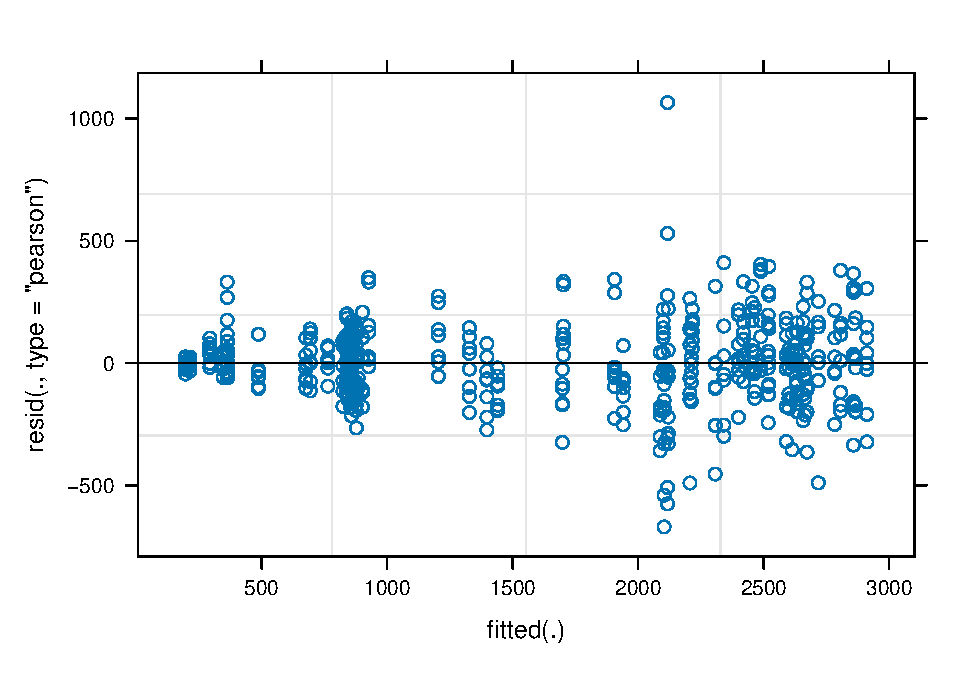
\includegraphics{for_markdown_files/figure-latex/unnamed-chunk-4-1.pdf}

\begin{Shaded}
\begin{Highlighting}[]
\NormalTok{mod\_sqrt }\SpecialCharTok{\%\textgreater{}\%} \FunctionTok{plot}\NormalTok{()}
\end{Highlighting}
\end{Shaded}

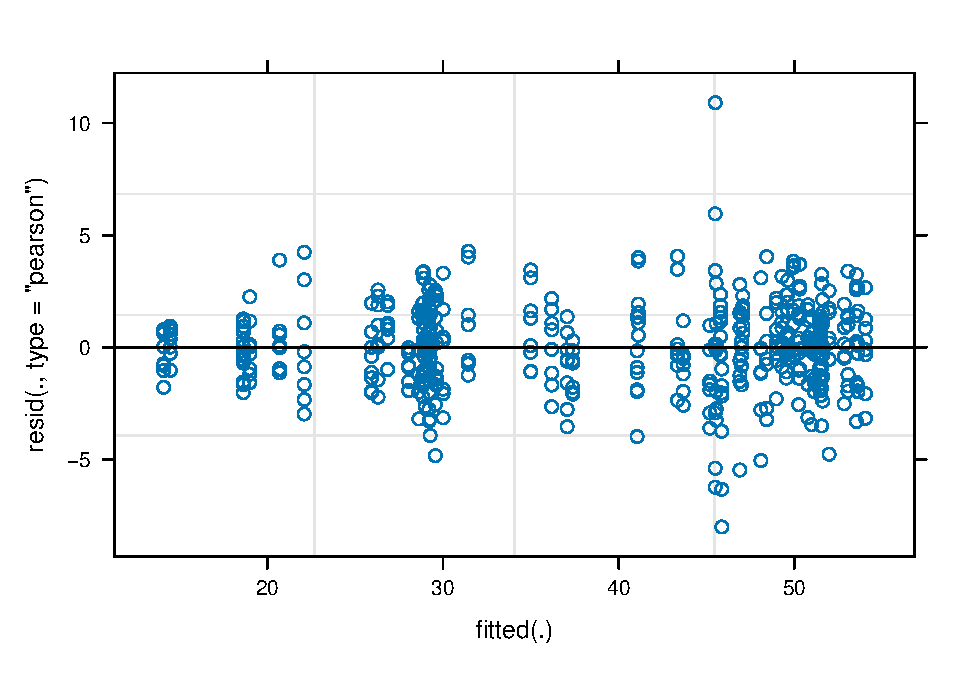
\includegraphics{for_markdown_files/figure-latex/unnamed-chunk-4-2.pdf}

\begin{Shaded}
\begin{Highlighting}[]
\NormalTok{mod\_log }\SpecialCharTok{\%\textgreater{}\%} \FunctionTok{plot}\NormalTok{()}
\end{Highlighting}
\end{Shaded}

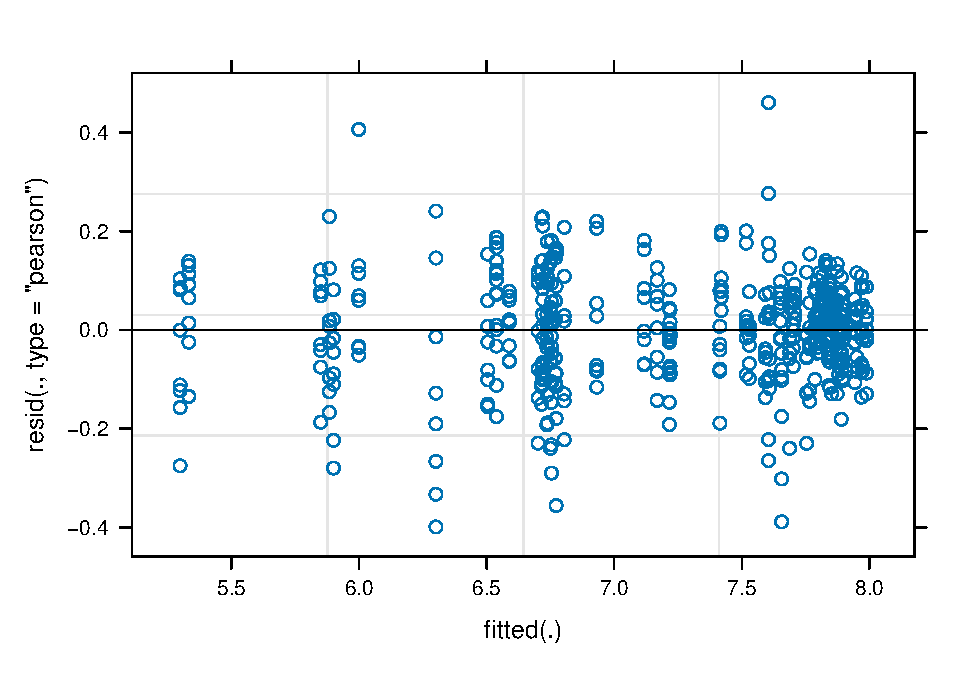
\includegraphics{for_markdown_files/figure-latex/unnamed-chunk-4-3.pdf}
We go log

\hypertarget{section-2}{%
\subsubsection{4.}\label{section-2}}

\begin{Shaded}
\begin{Highlighting}[]
\NormalTok{new\_mod }\OtherTok{\textless{}{-}} \FunctionTok{lme}\NormalTok{(fluorescence }\SpecialCharTok{\textasciitilde{}}\NormalTok{ day}\SpecialCharTok{*}\NormalTok{concFac, }\AttributeTok{random=}\SpecialCharTok{\textasciitilde{}}\DecValTok{1}\SpecialCharTok{|}\NormalTok{plate, }\AttributeTok{data=}\NormalTok{toxData,}
\AttributeTok{weights =} \FunctionTok{varPower}\NormalTok{(}\AttributeTok{form=}\SpecialCharTok{\textasciitilde{}}\FunctionTok{fitted}\NormalTok{(.)))}
\NormalTok{new\_mod }\SpecialCharTok{\%\textgreater{}\%} \FunctionTok{plot}\NormalTok{()}
\end{Highlighting}
\end{Shaded}

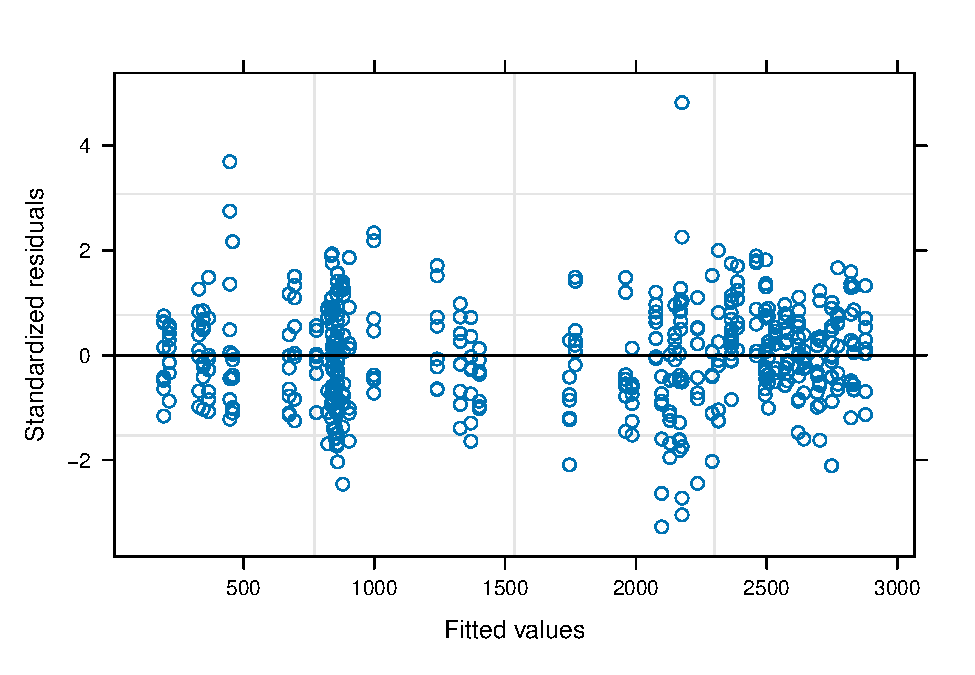
\includegraphics{for_markdown_files/figure-latex/unnamed-chunk-5-1.pdf}

\begin{Shaded}
\begin{Highlighting}[]
\FunctionTok{summary}\NormalTok{(new\_mod)}
\end{Highlighting}
\end{Shaded}

\begin{verbatim}
## Linear mixed-effects model fit by REML
##   Data: toxData 
##        AIC      BIC    logLik
##   6218.882 6343.527 -3079.441
## 
## Random effects:
##  Formula: ~1 | plate
##         (Intercept)  Residual
## StdDev:    159.7021 0.8225523
## 
## Variance function:
##  Structure: Power of variance covariate
##  Formula: ~fitted(.) 
##  Parameter estimates:
##     power 
## 0.7202027 
## Fixed effects:  fluorescence ~ day * concFac 
##                         Value Std.Error  DF    t-value p-value
## (Intercept)          893.0931 116.67283 467   7.654679  0.0000
## day2                1481.5202 155.39486   4   9.533907  0.0007
## day3                1665.6699 172.59820   4   9.650564  0.0006
## concFac0.005         -24.4782  39.79025 467  -0.615181  0.5387
## concFac0.0158        -44.5094  39.48871 467  -1.127143  0.2603
## concFac0.05          -44.1773  39.49370 467  -1.118591  0.2639
## concFac0.158         -47.0214  39.45096 467  -1.191896  0.2339
## concFac0.5           -60.5521  39.24781 467  -1.542814  0.1236
## concFac1.58         -208.8120  37.05301 467  -5.635495  0.0000
## concFac5            -537.4895  32.55303 467 -16.511199  0.0000
## concFac15.8         -688.1037  30.82601 467 -22.322181  0.0000
## day2:concFac0.005   -337.3375  73.74311 467  -4.574496  0.0000
## day3:concFac0.005    223.3352  93.93503 467   2.377549  0.0178
## day2:concFac0.0158  -124.6180  73.58821 467  -1.693451  0.0910
## day3:concFac0.0158   192.9133  93.27167 467   2.068295  0.0392
## day2:concFac0.05    -100.6919  73.79072 467  -1.364561  0.1730
## day3:concFac0.05     298.5788  94.40136 467   3.162865  0.0017
## day2:concFac0.158     83.6430  75.27540 467   1.111160  0.2671
## day3:concFac0.158    256.6344  93.90627 467   2.732878  0.0065
## day2:concFac0.5      106.8776  75.25042 467   1.420293  0.1562
## day3:concFac0.5      187.0477  92.93732 467   2.012622  0.0447
## day2:concFac1.58    -175.0767  71.10738 467  -2.462145  0.0142
## day3:concFac1.58     -49.3415  87.95306 467  -0.560998  0.5751
## day2:concFac5       -594.6452  62.20532 467  -9.559394  0.0000
## day3:concFac5       -716.6774  76.01794 467  -9.427741  0.0000
## day2:concFac15.8    -994.5789  57.40552 467 -17.325493  0.0000
## day3:concFac15.8   -1477.4286  67.83022 467 -21.781275  0.0000
##  Correlation: 
##                    (Intr) day2   day3   cF0.00 cF0.01 cF0.05 cF0.15 cnF0.5
## day2               -0.751                                                 
## day3               -0.676  0.508                                          
## concFac0.005       -0.185  0.139  0.125                                   
## concFac0.0158      -0.187  0.140  0.126  0.547                            
## concFac0.05        -0.187  0.140  0.126  0.547  0.552                     
## concFac0.158       -0.187  0.140  0.126  0.548  0.552  0.552              
## concFac0.5         -0.188  0.141  0.127  0.551  0.555  0.555  0.556       
## concFac1.58        -0.199  0.149  0.134  0.583  0.588  0.588  0.588  0.591
## concFac5           -0.226  0.170  0.153  0.664  0.669  0.669  0.670  0.673
## concFac15.8        -0.239  0.180  0.162  0.701  0.707  0.707  0.707  0.711
## day2:concFac0.005   0.100 -0.252 -0.068 -0.540 -0.295 -0.295 -0.296 -0.297
## day3:concFac0.005   0.078 -0.059 -0.264 -0.424 -0.232 -0.232 -0.232 -0.233
## day2:concFac0.0158  0.100 -0.253 -0.068 -0.294 -0.537 -0.296 -0.296 -0.298
## day3:concFac0.0158  0.079 -0.059 -0.266 -0.232 -0.423 -0.234 -0.234 -0.235
## day2:concFac0.05    0.100 -0.252 -0.068 -0.293 -0.295 -0.535 -0.295 -0.297
## day3:concFac0.05    0.078 -0.059 -0.263 -0.229 -0.231 -0.418 -0.231 -0.232
## day2:concFac0.158   0.098 -0.247 -0.066 -0.287 -0.289 -0.289 -0.524 -0.291
## day3:concFac0.158   0.079 -0.059 -0.264 -0.230 -0.232 -0.232 -0.420 -0.233
## day2:concFac0.5     0.098 -0.247 -0.066 -0.287 -0.289 -0.289 -0.290 -0.522
## day3:concFac0.5     0.079 -0.060 -0.267 -0.233 -0.234 -0.234 -0.235 -0.422
## day2:concFac1.58    0.104 -0.262 -0.070 -0.304 -0.306 -0.306 -0.307 -0.308
## day3:concFac1.58    0.084 -0.063 -0.282 -0.246 -0.248 -0.248 -0.248 -0.249
## day2:concFac5       0.119 -0.299 -0.080 -0.348 -0.350 -0.350 -0.351 -0.352
## day3:concFac5       0.097 -0.073 -0.327 -0.284 -0.287 -0.287 -0.287 -0.288
## day2:concFac15.8    0.128 -0.324 -0.087 -0.377 -0.379 -0.379 -0.380 -0.382
## day3:concFac15.8    0.109 -0.082 -0.366 -0.319 -0.321 -0.321 -0.321 -0.323
##                    cF1.58 cncFc5 cF15.8 d2:F0.00 d3:F0.00 d2:F0.01 d3:F0.01
## day2                                                                       
## day3                                                                       
## concFac0.005                                                               
## concFac0.0158                                                              
## concFac0.05                                                                
## concFac0.158                                                               
## concFac0.5                                                                 
## concFac1.58                                                                
## concFac5            0.713                                                  
## concFac15.8         0.753  0.857                                           
## day2:concFac0.005  -0.315 -0.358 -0.378                                    
## day3:concFac0.005  -0.247 -0.281 -0.297  0.229                             
## day2:concFac0.0158 -0.315 -0.359 -0.379  0.533    0.124                    
## day3:concFac0.0158 -0.249 -0.283 -0.299  0.125    0.489    0.227           
## day2:concFac0.05   -0.315 -0.358 -0.378  0.532    0.124    0.533    0.125  
## day3:concFac0.05   -0.246 -0.280 -0.296  0.124    0.483    0.124    0.487  
## day2:concFac0.158  -0.308 -0.351 -0.371  0.521    0.122    0.522    0.123  
## day3:concFac0.158  -0.247 -0.281 -0.297  0.124    0.486    0.124    0.489  
## day2:concFac0.5    -0.308 -0.351 -0.371  0.521    0.122    0.522    0.123  
## day3:concFac0.5    -0.250 -0.284 -0.300  0.126    0.491    0.126    0.494  
## day2:concFac1.58   -0.521 -0.372 -0.392  0.552    0.129    0.553    0.130  
## day3:concFac1.58   -0.421 -0.300 -0.317  0.133    0.519    0.133    0.522  
## day2:concFac5      -0.373 -0.523 -0.449  0.631    0.147    0.632    0.148  
## day3:concFac5      -0.305 -0.428 -0.367  0.153    0.600    0.154    0.604  
## day2:concFac15.8   -0.404 -0.460 -0.537  0.683    0.160    0.685    0.161  
## day3:concFac15.8   -0.342 -0.390 -0.454  0.172    0.673    0.172    0.677  
##                    d2:F0.05 d3:F0.05 d2:F0.1 d3:F0.1 d2:F0.5 d3:F0.5 d2:F1.
## day2                                                                       
## day3                                                                       
## concFac0.005                                                               
## concFac0.0158                                                              
## concFac0.05                                                                
## concFac0.158                                                               
## concFac0.5                                                                 
## concFac1.58                                                                
## concFac5                                                                   
## concFac15.8                                                                
## day2:concFac0.005                                                          
## day3:concFac0.005                                                          
## day2:concFac0.0158                                                         
## day3:concFac0.0158                                                         
## day2:concFac0.05                                                           
## day3:concFac0.05    0.224                                                  
## day2:concFac0.158   0.521    0.121                                         
## day3:concFac0.158   0.124    0.483    0.220                                
## day2:concFac0.5     0.521    0.121    0.511   0.122                        
## day3:concFac0.5     0.125    0.488    0.123   0.491   0.220                
## day2:concFac1.58    0.551    0.128    0.540   0.129   0.541   0.130        
## day3:concFac1.58    0.133    0.516    0.130   0.519   0.130   0.524   0.220
## day2:concFac5       0.630    0.146    0.618   0.147   0.618   0.149   0.654
## day3:concFac5       0.153    0.597    0.150   0.600   0.150   0.607   0.159
## day2:concFac15.8    0.683    0.159    0.669   0.160   0.670   0.161   0.708
## day3:concFac15.8    0.172    0.669    0.168   0.673   0.169   0.680   0.178
##                    d3:F1. dy2:F5 dy3:F5 d2:F15
## day2                                          
## day3                                          
## concFac0.005                                  
## concFac0.0158                                 
## concFac0.05                                   
## concFac0.158                                  
## concFac0.5                                    
## concFac1.58                                   
## concFac5                                      
## concFac15.8                                   
## day2:concFac0.005                             
## day3:concFac0.005                             
## day2:concFac0.0158                            
## day3:concFac0.0158                            
## day2:concFac0.05                              
## day3:concFac0.05                              
## day2:concFac0.158                             
## day3:concFac0.158                             
## day2:concFac0.5                               
## day3:concFac0.5                               
## day2:concFac1.58                              
## day3:concFac1.58                              
## day2:concFac5       0.157                     
## day3:concFac5       0.641  0.224              
## day2:concFac15.8    0.170  0.811  0.197       
## day3:concFac15.8    0.718  0.204  0.831  0.244
## 
## Standardized Within-Group Residuals:
##          Min           Q1          Med           Q3          Max 
## -3.278168327 -0.648805182 -0.009855112  0.634164702  4.823772219 
## 
## Number of Observations: 498
## Number of Groups: 7
\end{verbatim}

We go log still

\hypertarget{section-3}{%
\subsection{5.}\label{section-3}}

Estimates

\begin{Shaded}
\begin{Highlighting}[]
\NormalTok{reparm\_log }\OtherTok{\textless{}{-}} \FunctionTok{lmer}\NormalTok{(}\FunctionTok{log}\NormalTok{(fluorescence) }\SpecialCharTok{\textasciitilde{}}\NormalTok{ day}\SpecialCharTok{*}\NormalTok{concFac}\DecValTok{{-}1} \SpecialCharTok{+}\NormalTok{ (}\DecValTok{1}\SpecialCharTok{|}\NormalTok{plate) , }\AttributeTok{data =}\NormalTok{ toxData)}
\NormalTok{(reparm\_log }\SpecialCharTok{\%\textgreater{}\%} \FunctionTok{fixef}\NormalTok{())[}\FunctionTok{c}\NormalTok{(}\DecValTok{1}\NormalTok{,}\DecValTok{2}\NormalTok{,}\DecValTok{3}\NormalTok{)] }\SpecialCharTok{\%\textgreater{}\%} \FunctionTok{exp}\NormalTok{()}
\end{Highlighting}
\end{Shaded}

\begin{verbatim}
##      day1      day2      day3 
##  886.2118 2361.3400 2554.9882
\end{verbatim}

confints. This is the median.

\begin{Shaded}
\begin{Highlighting}[]
\NormalTok{((reparm\_log }\SpecialCharTok{\%\textgreater{}\%} \FunctionTok{confint}\NormalTok{()))[}\FunctionTok{c}\NormalTok{(}\DecValTok{3}\NormalTok{,}\DecValTok{4}\NormalTok{,}\DecValTok{5}\NormalTok{),] }\SpecialCharTok{\%\textgreater{}\%} \FunctionTok{exp}\NormalTok{()}
\end{Highlighting}
\end{Shaded}

\begin{verbatim}
## Computing profile confidence intervals ...
\end{verbatim}

\begin{verbatim}
##          2.5 %   97.5 %
## day1  764.2077 1027.694
## day2 2094.2014 2662.555
## day3 2205.6196 2959.697
\end{verbatim}

\begin{Shaded}
\begin{Highlighting}[]
\NormalTok{toxData }\SpecialCharTok{\%\textgreater{}\%} \FunctionTok{ggplot}\NormalTok{(}\FunctionTok{aes}\NormalTok{(}\AttributeTok{x =}\NormalTok{ concFac, }\AttributeTok{y =}\NormalTok{ fluorescence, }\AttributeTok{color =}\NormalTok{ day)) }\SpecialCharTok{+} \FunctionTok{geom\_point}\NormalTok{() }\SpecialCharTok{+} \FunctionTok{geom\_smooth}\NormalTok{(}\AttributeTok{method=}\StringTok{"lm"}\NormalTok{) }\SpecialCharTok{+} \FunctionTok{facet\_wrap}\NormalTok{(}\SpecialCharTok{\textasciitilde{}}\NormalTok{plate)}
\end{Highlighting}
\end{Shaded}

\begin{verbatim}
## `geom_smooth()` using formula = 'y ~ x'
\end{verbatim}

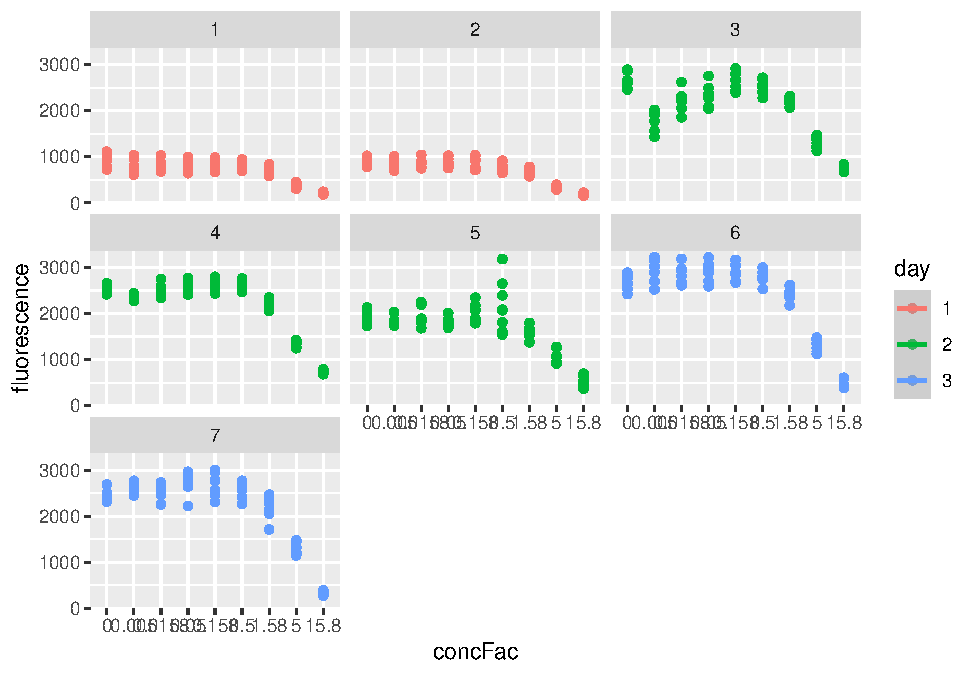
\includegraphics{for_markdown_files/figure-latex/unnamed-chunk-8-1.pdf}
\#\# 6

Want the concentration that gives half fluoresence corresponding to the
baseline conc. \[
E(\log(f_b/2)) = E(log(f_b))-\log(2)   
\]

\hypertarget{part-iii}{%
\subsection{Part III}\label{part-iii}}

\hypertarget{section-4}{%
\subsubsection{8.}\label{section-4}}

math. \(B_i\) are estimates of EC50 per day and \(D_i\) are estimates
for baseline per day.

\hypertarget{section-5}{%
\subsubsection{9.}\label{section-5}}

\hypertarget{section-6}{%
\subsection{10.}\label{section-6}}

\hypertarget{iv}{%
\subsection{IV}\label{iv}}

\hypertarget{section-7}{%
\subsubsection{11}\label{section-7}}

\begin{Shaded}
\begin{Highlighting}[]
\FunctionTok{library}\NormalTok{(rstan)}
\end{Highlighting}
\end{Shaded}

\begin{verbatim}
## Warning: package 'rstan' was built under R version 4.3.2
\end{verbatim}

\begin{verbatim}
## Loading required package: StanHeaders
\end{verbatim}

\begin{verbatim}
## Warning: package 'StanHeaders' was built under R version 4.3.2
\end{verbatim}

\begin{verbatim}
## 
## rstan version 2.32.3 (Stan version 2.26.1)
\end{verbatim}

\begin{verbatim}
## For execution on a local, multicore CPU with excess RAM we recommend calling
## options(mc.cores = parallel::detectCores()).
## To avoid recompilation of unchanged Stan programs, we recommend calling
## rstan_options(auto_write = TRUE)
## For within-chain threading using `reduce_sum()` or `map_rect()` Stan functions,
## change `threads_per_chain` option:
## rstan_options(threads_per_chain = 1)
\end{verbatim}

\begin{verbatim}
## Do not specify '-march=native' in 'LOCAL_CPPFLAGS' or a Makevars file
\end{verbatim}

\begin{Shaded}
\begin{Highlighting}[]
\NormalTok{to\_stan }\OtherTok{\textless{}{-}} \StringTok{"data \{}
\StringTok{int N;}
\StringTok{vector[N] day1dummy;}
\StringTok{vector[N] day2dummy;}
\StringTok{vector[N] day3dummy;}
\StringTok{vector[N] Z;}
\StringTok{vector[N] SE;}
\StringTok{\}}
\StringTok{parameters \{}
\StringTok{real theta\_1;}
\StringTok{real theta\_2;}
\StringTok{real theta\_3;}
\StringTok{real\textless{}lower = 0\textgreater{} tau;}
\StringTok{\}}
\StringTok{transformed parameters \{}
\StringTok{real ratio\_3\_1 = theta\_3/theta\_1;}
\StringTok{\}}
\StringTok{model \{}
\StringTok{Z \textasciitilde{} normal(theta\_1*day1dummy + theta\_2*day2dummy + theta\_3*day3dummy, sqrt(tau\^{}2 + SE\^{}2));}
\StringTok{\}}
\StringTok{"}
\FunctionTok{write}\NormalTok{(to\_stan, }\AttributeTok{file =} \StringTok{"model.stan"}\NormalTok{)}
\end{Highlighting}
\end{Shaded}

\begin{Shaded}
\begin{Highlighting}[]
\NormalTok{data }\OtherTok{\textless{}{-}} \FunctionTok{list}\NormalTok{(}\AttributeTok{N =} \FunctionTok{length}\NormalTok{(bData}\SpecialCharTok{$}\NormalTok{Estimate), }\AttributeTok{Z=}\NormalTok{bData}\SpecialCharTok{$}\NormalTok{Estimate, }\AttributeTok{day1dummy =}\NormalTok{ bData}\SpecialCharTok{$}\NormalTok{day1dummy, }
             \AttributeTok{day2dummy =}\NormalTok{ bData}\SpecialCharTok{$}\NormalTok{day2dummy, }\AttributeTok{day3dummy =}\NormalTok{ bData}\SpecialCharTok{$}\NormalTok{day3dummy, }\AttributeTok{SE =}\NormalTok{ bData}\SpecialCharTok{$}\NormalTok{SE)}
\NormalTok{fitted }\OtherTok{\textless{}{-}}\NormalTok{ rstan}\SpecialCharTok{::}\FunctionTok{stan}\NormalTok{(}\StringTok{"model.stan"}\NormalTok{, }\AttributeTok{data =}\NormalTok{ data, }\AttributeTok{iter =} \DecValTok{32000}\NormalTok{, }\AttributeTok{chains =} \DecValTok{4}\NormalTok{)}
\end{Highlighting}
\end{Shaded}

\begin{verbatim}
## 
## SAMPLING FOR MODEL 'anon_model' NOW (CHAIN 1).
## Chain 1: 
## Chain 1: Gradient evaluation took 4.9e-05 seconds
## Chain 1: 1000 transitions using 10 leapfrog steps per transition would take 0.49 seconds.
## Chain 1: Adjust your expectations accordingly!
## Chain 1: 
## Chain 1: 
## Chain 1: Iteration:     1 / 32000 [  0%]  (Warmup)
## Chain 1: Iteration:  3200 / 32000 [ 10%]  (Warmup)
## Chain 1: Iteration:  6400 / 32000 [ 20%]  (Warmup)
## Chain 1: Iteration:  9600 / 32000 [ 30%]  (Warmup)
## Chain 1: Iteration: 12800 / 32000 [ 40%]  (Warmup)
## Chain 1: Iteration: 16000 / 32000 [ 50%]  (Warmup)
## Chain 1: Iteration: 16001 / 32000 [ 50%]  (Sampling)
## Chain 1: Iteration: 19200 / 32000 [ 60%]  (Sampling)
## Chain 1: Iteration: 22400 / 32000 [ 70%]  (Sampling)
## Chain 1: Iteration: 25600 / 32000 [ 80%]  (Sampling)
## Chain 1: Iteration: 28800 / 32000 [ 90%]  (Sampling)
## Chain 1: Iteration: 32000 / 32000 [100%]  (Sampling)
## Chain 1: 
## Chain 1:  Elapsed Time: 2.36 seconds (Warm-up)
## Chain 1:                2.653 seconds (Sampling)
## Chain 1:                5.013 seconds (Total)
## Chain 1: 
## 
## SAMPLING FOR MODEL 'anon_model' NOW (CHAIN 2).
## Chain 2: 
## Chain 2: Gradient evaluation took 2.8e-05 seconds
## Chain 2: 1000 transitions using 10 leapfrog steps per transition would take 0.28 seconds.
## Chain 2: Adjust your expectations accordingly!
## Chain 2: 
## Chain 2: 
## Chain 2: Iteration:     1 / 32000 [  0%]  (Warmup)
## Chain 2: Iteration:  3200 / 32000 [ 10%]  (Warmup)
## Chain 2: Iteration:  6400 / 32000 [ 20%]  (Warmup)
## Chain 2: Iteration:  9600 / 32000 [ 30%]  (Warmup)
## Chain 2: Iteration: 12800 / 32000 [ 40%]  (Warmup)
## Chain 2: Iteration: 16000 / 32000 [ 50%]  (Warmup)
## Chain 2: Iteration: 16001 / 32000 [ 50%]  (Sampling)
## Chain 2: Iteration: 19200 / 32000 [ 60%]  (Sampling)
## Chain 2: Iteration: 22400 / 32000 [ 70%]  (Sampling)
## Chain 2: Iteration: 25600 / 32000 [ 80%]  (Sampling)
## Chain 2: Iteration: 28800 / 32000 [ 90%]  (Sampling)
## Chain 2: Iteration: 32000 / 32000 [100%]  (Sampling)
## Chain 2: 
## Chain 2:  Elapsed Time: 2.476 seconds (Warm-up)
## Chain 2:                3.057 seconds (Sampling)
## Chain 2:                5.533 seconds (Total)
## Chain 2: 
## 
## SAMPLING FOR MODEL 'anon_model' NOW (CHAIN 3).
## Chain 3: 
## Chain 3: Gradient evaluation took 2.4e-05 seconds
## Chain 3: 1000 transitions using 10 leapfrog steps per transition would take 0.24 seconds.
## Chain 3: Adjust your expectations accordingly!
## Chain 3: 
## Chain 3: 
## Chain 3: Iteration:     1 / 32000 [  0%]  (Warmup)
## Chain 3: Iteration:  3200 / 32000 [ 10%]  (Warmup)
## Chain 3: Iteration:  6400 / 32000 [ 20%]  (Warmup)
## Chain 3: Iteration:  9600 / 32000 [ 30%]  (Warmup)
## Chain 3: Iteration: 12800 / 32000 [ 40%]  (Warmup)
## Chain 3: Iteration: 16000 / 32000 [ 50%]  (Warmup)
## Chain 3: Iteration: 16001 / 32000 [ 50%]  (Sampling)
## Chain 3: Iteration: 19200 / 32000 [ 60%]  (Sampling)
## Chain 3: Iteration: 22400 / 32000 [ 70%]  (Sampling)
## Chain 3: Iteration: 25600 / 32000 [ 80%]  (Sampling)
## Chain 3: Iteration: 28800 / 32000 [ 90%]  (Sampling)
## Chain 3: Iteration: 32000 / 32000 [100%]  (Sampling)
## Chain 3: 
## Chain 3:  Elapsed Time: 2.377 seconds (Warm-up)
## Chain 3:                2.521 seconds (Sampling)
## Chain 3:                4.898 seconds (Total)
## Chain 3: 
## 
## SAMPLING FOR MODEL 'anon_model' NOW (CHAIN 4).
## Chain 4: 
## Chain 4: Gradient evaluation took 2.3e-05 seconds
## Chain 4: 1000 transitions using 10 leapfrog steps per transition would take 0.23 seconds.
## Chain 4: Adjust your expectations accordingly!
## Chain 4: 
## Chain 4: 
## Chain 4: Iteration:     1 / 32000 [  0%]  (Warmup)
## Chain 4: Iteration:  3200 / 32000 [ 10%]  (Warmup)
## Chain 4: Iteration:  6400 / 32000 [ 20%]  (Warmup)
## Chain 4: Iteration:  9600 / 32000 [ 30%]  (Warmup)
## Chain 4: Iteration: 12800 / 32000 [ 40%]  (Warmup)
## Chain 4: Iteration: 16000 / 32000 [ 50%]  (Warmup)
## Chain 4: Iteration: 16001 / 32000 [ 50%]  (Sampling)
## Chain 4: Iteration: 19200 / 32000 [ 60%]  (Sampling)
## Chain 4: Iteration: 22400 / 32000 [ 70%]  (Sampling)
## Chain 4: Iteration: 25600 / 32000 [ 80%]  (Sampling)
## Chain 4: Iteration: 28800 / 32000 [ 90%]  (Sampling)
## Chain 4: Iteration: 32000 / 32000 [100%]  (Sampling)
## Chain 4: 
## Chain 4:  Elapsed Time: 2.327 seconds (Warm-up)
## Chain 4:                2.714 seconds (Sampling)
## Chain 4:                5.041 seconds (Total)
## Chain 4:
\end{verbatim}

\begin{verbatim}
## Warning: There were 6 divergent transitions after warmup. See
## https://mc-stan.org/misc/warnings.html#divergent-transitions-after-warmup
## to find out why this is a problem and how to eliminate them.
\end{verbatim}

\begin{verbatim}
## Warning: Examine the pairs() plot to diagnose sampling problems
\end{verbatim}

\begin{Shaded}
\begin{Highlighting}[]
\NormalTok{fitted}
\end{Highlighting}
\end{Shaded}

\begin{verbatim}
## Inference for Stan model: anon_model.
## 4 chains, each with iter=32000; warmup=16000; thin=1; 
## post-warmup draws per chain=16000, total post-warmup draws=64000.
## 
##            mean se_mean   sd  2.5%   25%   50%   75% 97.5% n_eff Rhat
## theta_1    4.14    0.00 0.75  2.73  3.83  4.14  4.45  5.58 22860    1
## theta_2    6.62    0.00 0.65  5.46  6.31  6.60  6.91  7.87 29628    1
## theta_3    4.74    0.00 0.74  3.36  4.46  4.73  5.01  6.11 22372    1
## tau        0.70    0.01 0.75  0.03  0.28  0.53  0.89  2.39  8500    1
## ratio_3_1  1.17    0.01 3.55  0.71  1.04  1.14  1.26  1.82 65282    1
## lp__      -2.00    0.02 2.20 -7.69 -2.98 -1.44 -0.43  0.57  8710    1
## 
## Samples were drawn using NUTS(diag_e) at Fri Jan 12 10:43:38 2024.
## For each parameter, n_eff is a crude measure of effective sample size,
## and Rhat is the potential scale reduction factor on split chains (at 
## convergence, Rhat=1).
\end{verbatim}

\begin{Shaded}
\begin{Highlighting}[]
\FunctionTok{traceplot}\NormalTok{(fitted, }\AttributeTok{pars =} \FunctionTok{c}\NormalTok{(}\StringTok{"theta\_1"}\NormalTok{,}\StringTok{"theta\_2"}\NormalTok{,}\StringTok{"theta\_3"}\NormalTok{,}\StringTok{"tau"}\NormalTok{))}
\end{Highlighting}
\end{Shaded}

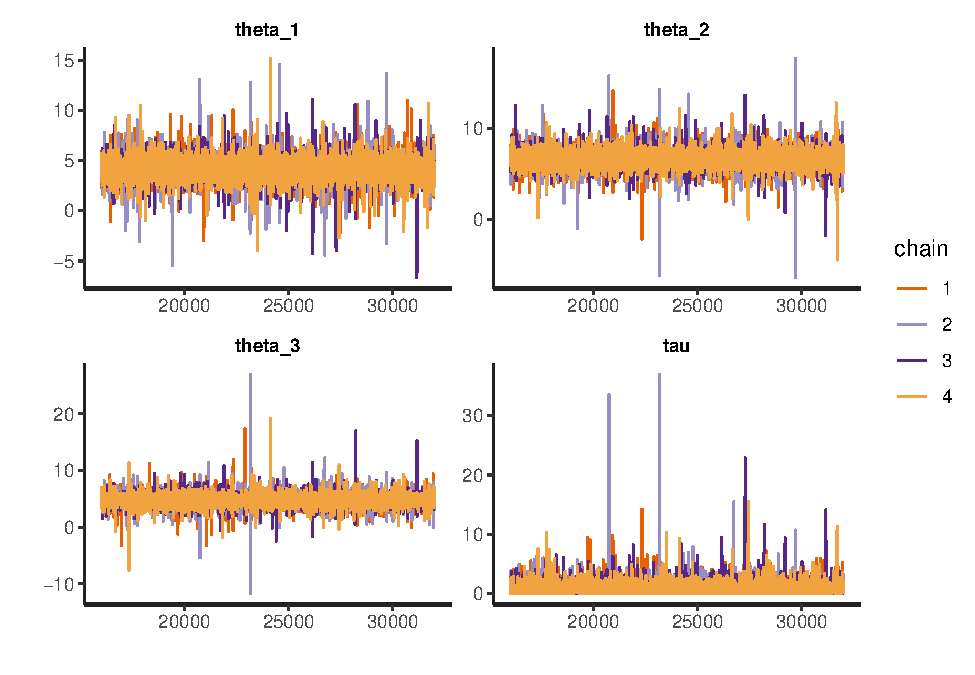
\includegraphics{for_markdown_files/figure-latex/unnamed-chunk-15-1.pdf}

\end{document}
